\question{Кинетический момент точки и системы относительно центра и оси.
Кинетический момент вращающегося твердого тела относительно оси вращения.
Теорема об изменении кинетического момента для точки.}

Рассмотрим систему материальных точек с массами \( m_1 \), \( m_2 \), \ldots,
\( m_n \), имеющих в данный момент скорости \( v_1 \), \( v_2 \), \ldots,
\( v_n \) относительно инерциальной системы отсчета. Выберем произвольный центр
\( O \) (рис. \ref{pic48_1}). Кинетическим моментом точки \( m_j \) относительно центра \( O \)
называется вектор момента её количества движения относительно этого центра:
\[
    \vec{k}_{O_j} = \vec{r}_j \times m_j\vec{v}_j.
\]

Известно, что векторное умножение можно записать через присоединенную матрицу
первого сомножителя -- радиуса вектора \( \vec{r} \). Опуская индекс, запишем
матричное выражение в осях \( xyz \) c началом в \( O \): \( K_O = mRv \), где
\( R \) -- антисимметричная присоединенная матрица вектора \( r \):
\[
    \begin{pmatrix} K_x \\ K_y \\ K_z \end{pmatrix} =
    m\begin{pmatrix} 0 & -z & y \\ z & 0 & -x \\ -y & x & 0 \end{pmatrix}
    \begin{pmatrix} \dot{x} \\ \dot{y} \\ \dot{z} \end{pmatrix} = 
    m\begin{pmatrix} y\dot{z} - z\dot{y} \\ z\dot{x} - x\dot{z} \\
    x\dot{y} - y\dot{x} \end{pmatrix}.
\]
 
Проекция кинетического момента на ось называются кинетическим моментом точки
относительно оси. Момент дает только касательная составляющая вектора
\( \vec{q} \) (рис. \ref{pic48_2}): \( k_z = \pm q_\tau h \).

Момент обращается в ноль, если вектор количества движения лежит в одной
плоскости с осью. Кинетическим моментом системы относительно центра \( O \)
называется главный момент количеств движений точек системы относительно этого
центра: \( \vec{K}_O = \sum \vec{k}_{O_j} = \sum m_j \vec{r}_j \times
\vec{v}_j \) или в матричной форме:
\[
    \begin{pmatrix} K_x \\ K_y \\ K_z \end{pmatrix} = \sum_j m_j
    \begin{pmatrix} y_j\dot{z}_j - z_j\dot{y}_j \\ z_j\dot{x}_j - x_j\dot{z}_j
    \\ x_j\dot{y}_j - y_j\dot{x}_j \end{pmatrix}
\]

\begin{figure}[h!]
    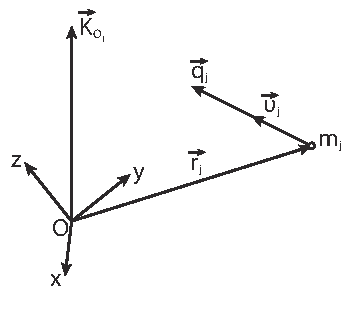
\includegraphics[width=.32\textwidth]{48_01}
    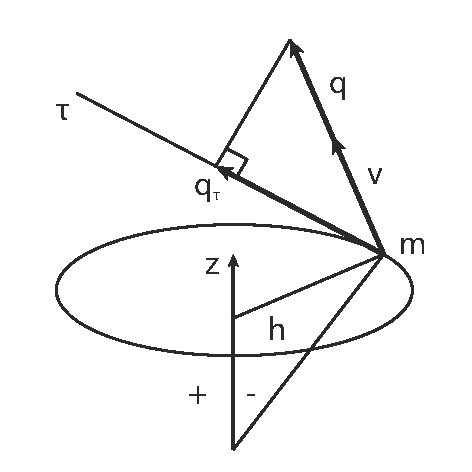
\includegraphics[width=.32\textwidth]{48_02}
    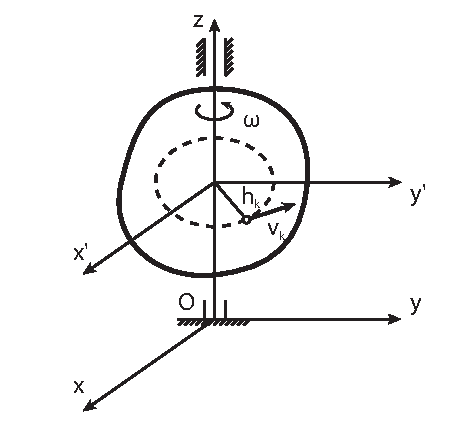
\includegraphics[width=.32\textwidth]{48_03} \\
    \parbox{.32\textwidth}{\caption{} \label{pic48_1}}
    \parbox{.32\textwidth}{\caption{} \label{pic48_2}}
    \parbox{.32\textwidth}{\caption{} \label{pic48_3}}
\end{figure}

Вычислим кинетический момент вращающегося вокруг оси тела (рис. \ref{pic48_3}). Пусть угловая
скорость тела будет \( \omega \), тогда для любой точки отстоящей от оси на
расстояние \( h_j \), скорость будет \( v_j = \omega h_j \), а момент
относительно \( Oz \):
\[
    \vec{k}_j = m_j v_j h_j = m_j\omega h_j^2.
\]

Подставляя это соотношение в \( K_x = \sum k_{x_j} \),
\( K_y = \sum k_{y_j} \), \( K_z = \sum k_{z_j} \) получаем:
\[
    K_z = \sum k_{z_j} = \sum (m_j h_j^2)\omega
\] 
или используя формулу \( I_z = \sum m_j h_j^2 \) (\( I \ge 0 \)):
\( K_z = I_z\omega \).
 
Кинетический момент вращающегося тела относительно оси вращения равен
произведению момента инерции тела относительно этой оси на угловую скорость
тела.

Если система состоит из нескольких тел, то:
\[
    K_z = I_{1_z}\omega_1 + I_{2_z}\omega_2 + \ldots + I_{N_z}\omega_N =
    \sum I_{j_z}\omega_j.
\]
 
Теорема моментов справедлива для каждой точки системы. Для одной точки:
\[
    \der{\vec{k}_{O_j}}{t} = \vec{m}^e_{O_j} +
    \vec{m}^i_{O_j}.
\]
Для всех точек:
\begin{gather*}
    \der{}{t}\left(\sum\vec{k}_{O_j}\right) =
    \sum\vec{m}^e_{O_j} + \sum\vec{m}^i_{O_j}, \\
    \der{\vec{K}_O}{t} = \sum\vec{m}^e_{O_j} = \vec{M}^e_O.
\end{gather*}

\newpage
